\chapter{Depth Profiling with XPS and AES}
In the previous chapters we have discussed the XPS and AES methods for surface analysis. Both methods are very useful for determination of the qualitative composition, although XPS clearly is the most advantageous for identifications of chemical composition and when an accurate quantitative determination is called for. On the other hand, AES is advantageous if information of the lateral composition is necessary. Both methods can also be used for a determination deeper into the material. We have already seen that some depth information can be obtained by tilting the sample relative to the analyser. This, however, only gives a depth resolution of a few atomic layers. Therefore, the methods must be combined with other methods so that the interesting layer can be exposed to the surface sensitive analysis. This can be done mechanically by a broad variety of polishing procedures or by sputtering.

\section{Instrumentation}
The first class of methods is the mechanical type where the interesting part of the sample can be exposed simply by making a cut orthogonal to the surface or by ball cratering. In the first case the deep lying layers can then be analysed by use of SAM (see Fig. \ref{fig:samorthcut}). It is immediately seen that the resolution of this analysis will be limited by the resolution of the SAM available. This may not be trivial as it is not always easy to prepare a sample with a perfect cut orthogonal to the surface, especially not in the cases where the region is very inhomogeneous. The ball cratering method, as shown in \autoref{fig:ballcrater}, is very similar except that a crater is polished in the surface. Different layers will then be exposed and can again be analysed by use of SAM with sufficient resolution.

In both cases the depth resolution is given by SAM (\SI{200}{\angstrom} and upwards), although it can be improved considerably in the ball cratering method due to the fact that we here have a cut under an angle. These methods are seldom used because in general it is much more convenient to use EDX on such samples.

\begin{figure}[h!]
	\begin{center}
	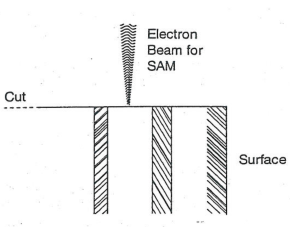
\includegraphics[scale=3]{figures/07_01.png}
	\caption{Sketch of SAM analysis of an orthogonal cut.}
	\label{fig:samorthcut}
	\end{center}
\end{figure}

\begin{figure}[h!]
	\begin{center}
	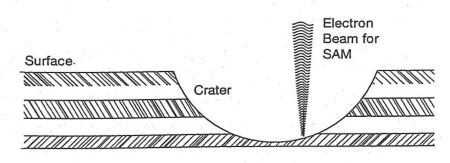
\includegraphics[scale=3]{figures/07_02.png}
	\caption{Sketch of the ball cratering method.}
	\label{fig:ballcrater}
	\end{center}
\end{figure}

However, in the range \SIrange{0}{1000}{\angstrom} there is another method by which the surface can easily be exposed and analysed by use of both AES or XPS, namely by sputtering with rare gas atoms, preferentially argon. By ionising Argon at a high potential the ions created can be manipulated just like the electrons and be focused into a spot on the surface and scanned if necessary. The formation of the beam is very similar to the way we measured the pressure in the chamber as shown in \autoref{fig:ion_gauge}. Instead of collecting the ions on the collector they are extracted from the cage formed by the grid and accelerated towards the sample which is usually kept grounded. In this manner ion beams with energies of \SIrange{1}{5}{k\electronvolt} and with currents of \SIrange{0}{10}{\micro A} can be formed. The argon is supplied by leaking in argon in the chamber to the required pressure of roughly \SI{1e-5}{mbar}. This is a high pressure in the context of UHV and might also cause problems for some types of pumps, like for instance the ion pumps, but as the gas is inert it does not influence the surface analysis if the argon is sufficiently clean. The pressure in the chamber can be reduced about three orders of magnitude if a differentially pumped ion gun is used instead. In this case a high pressure is still needed in the ionising region but the beam is then passing through a small hole into the main chamber. By pumping the ion-gun and the main chamber by separate pumps (differentially pumped) the pressure in the main chamber may be kept in the \SI{e-8}{mbar} region. The spot size diameter is, as for the electron beam, determined by the current density and will typically be on the order of \SI{100}{\micro m} in standard equipment. The beam can be scanned to give a homogeneous exposure over a rather large area ($\SI{10}{mm}\times\SI{10}{mm}$) of the surface so depth analysis with XPS can be carried out. For other applications, like for instance Secondary Ion Mass Spectroscopy (SIMS), the beam can be focused down to much smaller spots sizes.

\section{Ion Sputtering}
Several types of rare gases can be used for sputter profiling, but usually argon is the preferred gas as it is cheap to purify and has a high sputter yield. When a high energetic ion is hitting the surface the ion will be neutralised and transfer energy to the surface atoms through a number of essentially binary collisions. Some of the surface atoms will obtain sufficient energy and momentum to be able to escape the surface (see Fig. \ref{fig:sputtering}). The atoms which in this manner are scattered off the surface will mostly leave as neutral species and only a small fraction will survive as ions. Since the ions are essentially coming from the top most layer and since they are easily detected by a mass spectrometer this is a method very useful for determining the depth composition into the surface as the atoms are sputtered away. This method is called SIMS as mentioned above and can be carried out in small spots. The method is extremely sensitive (ppm level) but is rather difficult to quantify since the survival of the ions depend exponentially on the work function of the surface. For further details on this method we shall refer the reader to \cite{briggs2}. A method has been developed which overcomes this problem by detecting all the atoms coming off the surface. This is a much more reliable way to determine the surface depth composition. However, since this method relies on resonance ionisation by two lasers it is not economically viable.

Therefore, it is much more convenient to simply use either XPS, or preferentially AES, to measure what is left on the surface after a certain number of atoms have been sputtered away by bombarding the surface with energetic \ce{Ar+} ions. The measurements can be made simultaneously with sputtering or by alternating between sputtering and measuring. The AES method is the preferred method because it is in general much faster than the XPS method.

\begin{figure}[h!]
 	\begin{center}
 	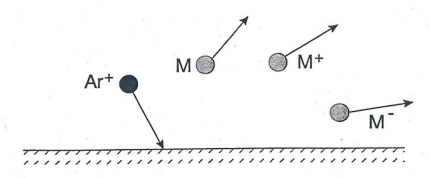
\includegraphics[scale=3]{figures/07_03.png}
 	\caption{Sketch of the sputtering process.}
 	\label{fig:sputtering}
 	\end{center}
 \end{figure} 

If we define a sputter yield $Y$ as the number of atoms removed from the surface per incoming ion it is possible, under ideal conditions, to convert time sputtered to a depth.

The flux of ions $F$ can be written as
 
\begin{equation}
F=\frac{I}{eA}
\end{equation}

\noindent where $I$ is the ion current and $A$ is the area exposed to the ion beam. In a pure element the number of atoms removed per second per area will be given by

\begin{equation}
g_i=FY_i
\end{equation}

$g_i$ can be converted to a depth by

\begin{equation}
\frac{dz_i}{dt}=\dot{z}_i=\frac{g_i}{N_i(z)}=\frac{FY_i(z)M_i}{\rho_i(z)N_A}=\frac{IY_i(z)M_i}{eA\rho_i(z)N_A}
\end{equation}

\noindent where $N_i$ is the density of atoms in the surface, $M_i$ is the mol weight, $N_A$ is Avogadro's number, and $\rho_i$ is the density of this particular element $i$. If we assume that $F$, $Y_i$, and $\rho_i$ are constants with respect to time this differential equation can easily be solved and the result is

\begin{equation}\label{eq:sputterdepth}
z(t)=\int_0^t\dot{z}dt=\frac{FYM}{\rho N_A}t=\frac{IYM}{eA\rho N_A}t
\end{equation}

This was a rather trivial example since it only applies for pure elements. Let us instead look at a two component mixture of $A$ and $B$ where we want to determine the depth compositions ($C_A(z)$ and $C_A(z)$). If we have two components, there will most likely be a difference in sputter yield for the two components leading to

\begin{equation}
z(t)=\int_0^t[C_A(t)\dot{z}_A+C_B(t)\dot{z}_B]dt 
\end{equation}

Since $C_A(z)$ and $C_A(z)$ can be estimated by the surface analysis as a function of time and since $\dot{z}$ can be estimated if the sputtering yield is known, it is possible to construct a plot showing the concentration profile of $A$ and $B$ into the material as a function of depth. Unfortunately it is generally not so simple since the sputtering yields for different compositions and compounds are not well known.

\subsection{The Sputter Yield}
The essential parameter for doing sputter profiling is the yield $Y$; the number of particles that is removed from the surface per incoming ion. The yield from a pure amorphous target can formally be written as

\begin{equation}
Y=\Delta F(E_0)
\end{equation}

\noindent where $\Delta$ is a factor containing all the material properties such as the surface binding energy of the atoms sputtered and $F(E_0)$ is the energy deposited at the surface depending upon the type of ions, the energy $E_0$, the incidence angle of the ions, the target atoms, and the density of the atoms in the target.

The parameter $\Delta$ can be derived describing the number of target atoms that obtains sufficient energy and momentum in the correct direction so that they can overcome the barrier and escape the surface. The result is

\begin{equation}
\Delta\approx\frac{0.042}{NU_0}
\end{equation}

in units of [\si{\angstrom /\electronvolt}] where $N$ [\si{\angstrom ^{-3}}] is the density of atoms in the target and $U_0$ [\si{\electronvolt}] is the surface binding energy of the target atoms. For details of the derivation of this expression we shall refer the reader to \cite{sigmund}. In \autoref{fig:xesputteryield} the sputter yield for \SI{400}{\electronvolt} \ce{Xe+} ions is plotted for most of the elements. It is clearly seen that there is a rather strong variation. More relevant data can be found in \cite{behrisch} where sputter yields for various ions, energies, and elements have been collected. All this works relatively well for the pure elements, but as soon as we turn to inhomogeneous samples consisting of alloys or compounds these sputter yields are in general not valid any longer since the surface binding energy changes for instance. Thus there is a general problem in converting the sputter time into a depth for more complex samples.

\begin{figure}[h!]
	\begin{center}
	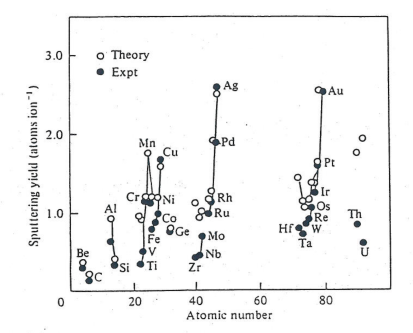
\includegraphics[scale=4]{figures/07_04.png}
	\caption{The sputter yield for \SI{500}{\electronvolt} Xe ions.}
	\label{fig:xesputteryield}
	\end{center}
\end{figure}

\section{Factors Limiting Depth Resolution and Accuracy of Profiles}
It is straight forward to perform a sputter profile and plot the concentration of the various components as a function of sputter time or even better as a function of ion dosage. The problem arises when we want to interpret these data in terms of depth and depth resolution.

\subsection{The Effect of Attenuation}
First of all, the AES-signals are not coming from a single layer but are exponentially damped signals from several layers. This means that we can never expect to obtain extremely sharp features, although the sample studied consists of such. Consider for example a thin layer of gold ($d_{\ce{Au}}=\SI{25}{\angstrom}$) deposited on top of a germanium surface and then covered by another layer of germanium $d_{\ce{Ge}}=\SI{30}{\angstrom}$. It is assumed that the deposition is ideal, i.e. it is a layer by layer growth mode (see Fig. \ref{fig:geattenuation}). We can easily adapt Equations \eqref{eq:gesignal} and \eqref{sisignal} to describe the intensities from the constructed sandwich. The signal from the gold will be given by

\begin{equation}
I_{\ce{Au}}=I^{\infty}_{\ce{Au}}\left(1-e^{-\dfrac{d_{\ce{Au}}}{\lambda_{\ce{Au} in \ce{Au}}}}\right)e^{-\dfrac{d_{\ce{Ge}}}{\lambda_{\ce{Au} in \ce{Ge}}}} 
\end{equation}

\noindent which is the gold signal from a gold layer of thickness $d_{\ce{Au}}$ damped through a germanium layer of thickness $d_{\ce{Ge}}$. The term $\lambda_{x in y}$ refers to the mean free path of an Auger electron from element $x$ moving through element $y$. Similarly, the signal from the germanium can be written as

\begin{equation}
I_{\ce{Ge}}=I^{\infty}_{\ce{Ge}}\left(1-e^{-\dfrac{d_{\ce{Ge}}}{\lambda_{\ce{Ge} in \ce{Ge}}}}\right)+ I^{\infty}_{\ce{Ge}}e^{-\dfrac{d_{\ce{Ge}}}{\lambda_{\ce{Ge} in \ce{Ge}}}-\dfrac{d_{\ce{Au}}}{\lambda_{\ce{Ge} in \ce{Au}}}}
\end{equation}

\noindent where the first term is due to the germanium overlayer and the second term is due to the germanium substrate which is damped both through the gold layer and the germanium overlayer.

This sandwich can now be analysed by sputter profiling. If it is assumed that the sputter profiling, just as the deposition, is ideal i.e. the removal takes place layer by layer it is easy to set up the equations describing the signals as a function of time. The sputter rate can be evaluated for each of the elements (Eq. \eqref{eq:sputterdepth}) and the thickness of the various layers can then be estimated as a function of time as $d-\dot{z}t$. If it takes $t_{\ce{Ge}}$ seconds to sputter through the germanium overlayer and $t_{\ce{Au}}$ for the gold layer the time dependence of the signals are naturally divided into two intervals. The signal for the gold layer is given by

\begin{equation}
I_{\ce{Au}}(t)=I^{\infty}_{\ce{Au}}\left(1-e^{-\dfrac{d_{\ce{Au}}}{\lambda_{\ce{Au} in \ce{Au}}}}\right)e^{-\dfrac{d_{\ce{Ge}}-\dot{z}_{\ce{Ge}} t}{\lambda_{\ce{Au} in \ce{Ge}}}} \hspace{2cm} 0\leq t\leq t_{\ce{Ge}}
\end{equation}

\noindent and

\begin{equation}
I_{\ce{Au}}(t)=I^{\infty}_{\ce{Au}}\left(1-e^{-\dfrac{d_{\ce{Au}}-\dot{z}_{\ce{Au}}(t-t_{\ce{Ge}})}{\lambda_{\ce{Au} in \ce{Au}}}}\right) \hspace{2cm} t_{\ce{Ge}}\leq t\leq t_{\ce{Ge}}+t_{\ce{Au}}
\end{equation}

The result for $(I_{\ce{Au}}(t)/I_{\ce{Au}}^{\infty})$ is plotted vs. sputter time for the values $\lambda_{\ce{Au} in \ce{Au}}=\SI{5}{\angstrom}$ and $\lambda_{\ce{Au} in \ce{Ge}}=\SI{10}{\angstrom}$ is shown in Figure 7.5. So even in this very ideal case the profile of the gold layer is broadened. Naturally it is possible to correct for this broadening as its origin is well understood. The above intensities are all special cases of

\begin{equation}
I_i=\frac{I^{\infty}_i}{\lambda_i}\int^{\infty}_0C_i(z\prime)e^{-\dfrac{z\prime}{\lambda_i}}dz\prime
\end{equation}

\noindent where $C_i(z\prime)$ is the concentration of element $i$ in depth $z$.

Ideally we started out with a concentration profile $C_i(z\prime)$ which in general is the unknown function we want to determine. The resulting intensity $I_i(z)$ where the sputter depth $z$ is a result of a convolution of a resolution function $g(z-z\prime)$ and the true concentration profile is thus

\begin{eqnarray}
I_i(z)	& =	& \frac{I^{\infty}_i}{\lambda_i}C_i(z\prime)*g(z-z')\\
I_i(z)	& =	& \frac{I^{\infty}_i}{\lambda_i} \int^{\infty}_{-\infty}C_i(z\prime)g(z-z\prime)dz\prime
\end{eqnarray}

So in this case where

\begin{equation}
g(z-z\prime)=e^{\frac{z-z\prime}{\lambda_i}}dz
\end{equation}

\noindent it is well established that a routine exists for elimination of this broadening. The broadening in the profile can as a rule of thumb be estimated as $\Delta z_{\lambda}=1.6\lambda$.

\begin{figure}[h!]
	\begin{center}
	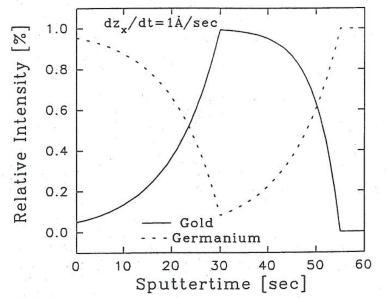
\includegraphics[scale=3.5]{figures/07_05.png}
	\caption{The relative intensity of gold from the sandwich as a function of sputter depth.}
	\label{fig:auint}
	\end{center}
\end{figure}

\subsection{Other Effects}
There are other effects leading both to broadening and shifts of the true profile which are not as easily dealt with. The sputtering process itself is quite a complex process and we shall here briefly mention a number of the effects that may lead to a broadening and introduce various errors when evaluating sputtering profiles.

\subsubsection{Statistical Broadening}
First of all the sputtering process is a random process, meaning that we should never expect to have a layer by layer removal. After some sputtering time we may have removed five layers off at one place of the surface, whereas seven layers have been removed at other places. This will lead to an additional broadening which is usually considered to be proportional to the square root of the depth in the region below \SI{100}{\angstrom}. For higher values of $z$, $\Delta z$ appears to saturate at roughly \SIrange{10}{20}{\angstrom}.

\subsubsection{Broadening by Surface Roughness}
Surface roughness will naturally also influence the resolution as will surface crystallography. Both effects can strongly influence the resolution as the sputter yield depends on the incoming angle of the ions. If for example a polycrystalline sample is sputtered for a long time, the sputtering itself may introduce structural changes of the surface leading to substantial broadening. This is clearly seen in \autoref{fig:emzi} where a polycrystalline zinc sample has been sputtered to a depth of \SIrange{3}{4}{\micro m} and subsequently studied by electron microscopy.

\begin{figure}[h!]
	\begin{center}
	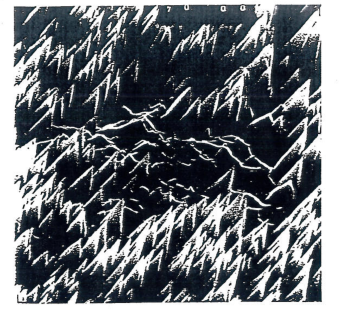
\includegraphics[scale=4]{figures/07_06.png}
	\caption{Electron microscope picture of a
 polycrystalline zinc sample sputtered to \SIrange{3}{4}{\micro m} depth.}
	\label{fig:emzi}
	\end{center}
\end{figure}

The surface which initially appeared flat is now extremely rough and it is clear that any concentration profiles measured on such a surface will be completely smeared out. This problem can to some extent be eliminated by averaging the incidence angle of the ion beam by rotating the sample during the sputtering process. The effect is shown in \autoref{fig:nicrsputter} where a sputter profile of a multi sandwich of Cr/Ni (each layer \SI{500}{\angstrom} thick) has been analysed with and without rotating the sample. The incident beam was \ce{Ar+} ions at \SI{1}{k\electronvolt} at an incidence angle of \ang{68} \cite{zalar}. The depth resolution for the rotated sample is clearly improved as seen in the lower panel of \autoref{fig:nicrsputter}.

\begin{figure}[h!]
	\begin{center}
	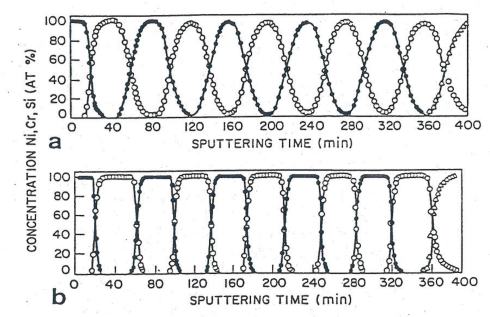
\includegraphics[scale=3.5]{figures/07_07.png}
	\caption{Sputter profile of a multi Ni/Cr sandwich without (top panel) and with (lower panel) simultaneous rotation of the sample.}
	\label{fig:nicrsputter}
	\end{center}
\end{figure}

\subsubsection{Preferential Sputtering}
If there is a large difference in sputter yield for the various components in the sample the surface concentration of the components may be changed due to the sputtering. Thus the surface composition will change from its true value to a composition determined by the steady state solution of the removal rates of the various components. This leads to an enrichment of the component which has the lower sputter yield and the sputter profiling will reflect a too high concentration of this particular component.

\subsubsection{Recoil Mixing}
The high energy ions hitting the surface will transfer energy and momentum to the surface atoms whereby there will be a mixing of the atoms at the surface. This in itself leads to a broadening of the profiles, but furthermore there will also be a possibility that some atoms are recoiled into the surface. This will result in a shift of the profiles to higher depths as some of the atoms are recoiled further into the sample before they are removed.

\subsubsection{Radiation Enhanced Diffusion and Segregation}
These effects both lead to broadening and errors in the concentration profiles. Due to the many defects the sputtering inevitably introduces in the surface region it will be much easier for the atoms to diffuse around. Thus if there is a component which has a very low surface energy, this component will prefer to segregate to the surface and cause an enrichment here which does not reflect the true composition of the sample. Similarly, any sharp interface will be smeared out by diffusion.

Several of the above effects will lead to broadening and as they all have to be convoluted it is appropriate to approximate the resolution function by a Gaussian

\begin{equation}
g(z-z\prime)=\frac{\pi \Delta z^2}{2}e^{-2\left(\dfrac{(z\prime-z)}{\Delta z}\right)^2}
\end{equation}

In general the resolution will decrease with depth as several of the discussed broadening effects are proportional to the depth sputtered. For a more detailed and rigorous treatment of the above discussed effects, the reader is referred to an excellent review by Hoffman \cite{hoffman} and references therein.

\section{Practical Sputter Profiling}
It is seen that there are many effects which make an accurate interpretation of a sputter profile a difficult task, even in cases where sandwiches of pure elements are studied. Sputter profiles are therefore generally presented as concentration profiles as a function of ion dosage. This is often sufficient as in many cases it is only necessary to discuss qualitative differences between different samples. In the following we shall go through a few such examples.

\subsection{Sputter Profile of Stainless Steel}
In \autoref{fig:sssputter} and \autoref{fig:ssheatsputter} the sputter profiles of a 18-8 stainless steel sample are shown just after it had been cut off a rod and after a heat treatment at \SI{600}{\degreeCelsius} for 600 seconds respectively.

\begin{figure}[h!]
	\begin{center}
	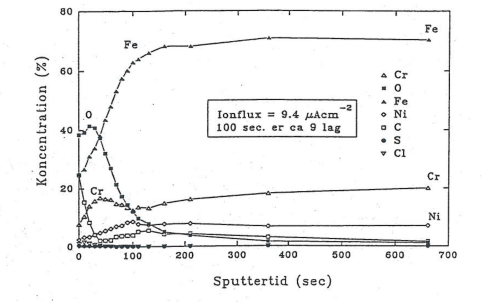
\includegraphics[scale=4]{figures/07_08.png}
	\caption{Sputter profile of stainless steel.}
	\label{fig:sssputter}
	\end{center}
\end{figure}

\begin{figure}[h!]
	\begin{center}
	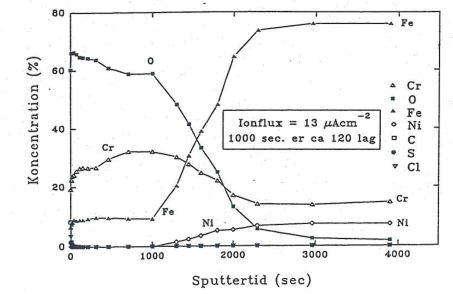
\includegraphics[scale=4]{figures/07_09.png}
	\caption{Sputter profile of heat treated
 stainless steel.}
	\label{fig:ssheatsputter}
	\end{center}
\end{figure}

In both cases a carbon contamination was observed at the surface prior to sputtering. Such a thin layer of surface contamination, is always observed on a sample that has been introduced into the apparatus from atmospheric pressure. It is readily removed after 10-20 seconds of sputtering. Also other forms of contamination like sulphur and chlorine can be observed. It is noticed that even on the non-treated surface (Fig. \ref{fig:sssputter}) there is a substantial oxide layer and an enrichment of chromium at the cost of iron and nickel in the surface region. This enrichment is further developed when the sample has been heated in atmospheric air at \SI{600}{\degreeCelsius} for 600 seconds as shown in \autoref{fig:ssheatsputter}. The surface layer can be identified by XPS as seen in \autoref{fig:ssxps} and consists mainly of \ce{Cr2O3} although less than \SI{10}{\percent} iron can still be observed.

\begin{figure}[h!]
	\begin{center}
	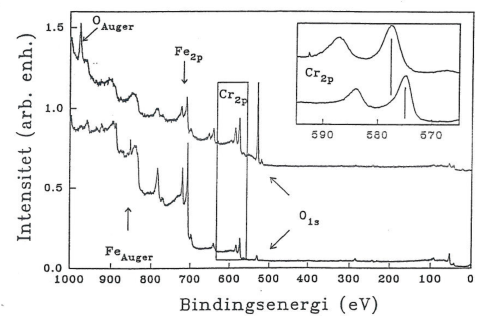
\includegraphics[scale=4]{figures/07_10.png}
	\caption{XPS spectra of the stainless steel sample before and after sputtering.}
	\label{fig:ssxps}
	\end{center}
\end{figure}

Approximately \SIrange{500}{1000}{\angstrom} must be removed before bulk values of the components are observed. The fact that it is chromium which is forming the protective oxide layer on the steel is in good agreement with the rule of thump that it is always the most reactive component which will segregate to the surface region and be oxidised. The reactivity of the transition metals is increasing from the right to the left. Therefore, if titanium had been present in the steel we would expect this to form an oxide overlayer as well. This simple picture holds well as long as the oxide layer grown is not too thick. For very thick layers (several \si{\micro m}) formed at high temperatures, the process becomes much more complex and NiO overlayers may be observed on top of the \ce{Cr2O3} \cite{alstrup}.

\subsection{Investigations of Electrical Contacts}
It has been mentioned that a substantial amount of all analysis performed by use of XPS and especially AES is done within the field of microelectronics. There are several problems which can be advantageously investigated with these methods and one of them is the formation of good contacts to the various semiconductors. Here we have chosen to show the contact formation to silicon. Gold usually forms good electrical contacts, but if it is deposited directly on the silicon it will readily diffuse into the silicon and be diluted. Therefore a layer of chromium is deposited on the silicon prior to the gold deposition. In \autoref{fig:aucrsisputter} the sputter profile of the contact is shown as deposited. In order to simulate ageing and use of the component it has been heated to \SI{300}{\degreeCelsius} for two hours and the result is shown in \autoref{fig:aucrsiheatsputter} where it is clearly seen that the chromium layer itself is not a sufficient diffusion barrier since silicon is observed in the gold overlayer and vice versa. If the procedure is repeated but the chromium is deposited in a background gas of nitrogen some chromium nitride will be formed as shown in \autoref{fig:aucrnsisputter}. Performing the same ageing experiment clearly shows (see Fig. \ref{fig:aucrnsiheatsputter}) that this construction is much better since the mixing has been minimised. Thus, the chromium nitride forms a diffusion barrier for gold and silicon.

\subsection{Control of Thin Coatings}
Coatings are used widely in industrial processes mainly for corrosion protection or for chemical inertness. In the latter case it is very common to deposit a thin layer of gold on the surface. For example many metals that are used for bijouterie and the rim of glasses will contain nickel. This is a highly non-desirable situation for metals in contact with the human body since it may cause allergic reactions. On the other hand, gold is a rather expensive material so the manufacturer wants to keep the layer as thin as possible. \autoref{fig:aunisputter} shows a sputter profile of a sample where the manufacturer was cutting the expenses too low since he was not successful in avoiding nickel at the surface. Only a few hundred \si{\angstrom} of gold had been deposited and since gold in this sort of industrial process is usually growing in an island growth mode, there will be areas free of gold exposing the nickel.

\begin{figure}[h!]
	\begin{center}
	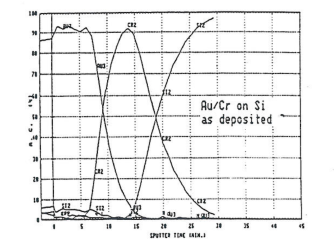
\includegraphics[scale=4.5]{figures/07_11a.png}
	\caption{Sputter profile of gold film on chromium on silicon as deposited.}
	\label{fig:aucrsisputter}
	\end{center}
\end{figure}

\begin{figure}[h!]
	\begin{center}
	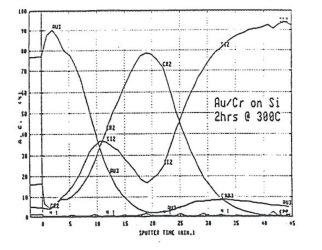
\includegraphics[scale=4.5]{figures/07_11b.png}
	\caption{Sputter profile of gold film on chromium on silicon heat treated to \SI{300}{\degreeCelsius} for two hours.}
	\label{fig:aucrsiheatsputter}
	\end{center}
\end{figure}

\begin{figure}[h!]
	\begin{center}
	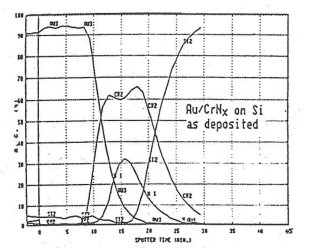
\includegraphics[scale=4.5]{figures/07_12a.png}
	\caption{Sputter profile of gold film on chromium-nitride on silicon as deposited.}
	\label{fig:aucrnsisputter}
	\end{center}
\end{figure}

\begin{figure}[h!]
	\begin{center}
	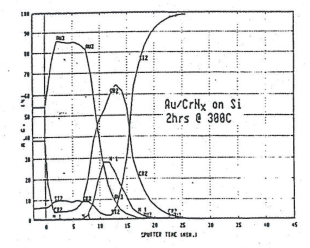
\includegraphics[scale=4.5]{figures/07_12b.png}
	\caption{Sputter profile of gold film on chromium-nitride on silicon heat treated to \SI{300}{\degreeCelsius} for two hours.}
	\label{fig:aucrnsiheatsputter}
	\end{center}
\end{figure}

\begin{figure}[h!]
 	\begin{center}
 	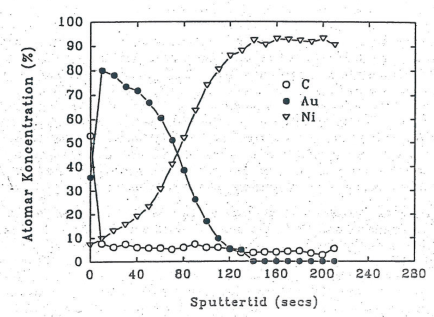
\includegraphics[scale=4]{figures/07_13.png}
 	\caption{Sputter profile of a glass rim consisting of nickel coated with gold.}
 	\label{fig:aunisputter}
 	\end{center}
\end{figure} 

\newpage
\section{Problems}
\begin{enumerate}
\item In the semiconductor industry it is often a requirement to be able to make good electrical contact to silicon wafers. This is often done by evaporating a thin film of gold upon the silicon. The evaporation rate is, however, in our case not known. The rate is, therefore, estimated by sputter profiling, that is measuring the surface composition while bombarding it with \SI{2.0}{k\electronvolt} Ar ions. The ion fluency is measured to be \SI{5}{\micro A/cm^2}. It takes 22 minutes before the gold disappears and the silicon appears. This is idealised, how does it look in reality?. The sputter yield has earlier been determined to be 2.6 Au atoms per Ar ion. Determine the thickness of the gold overlayer. How long time will it take to sputter through a silicon layer of a similar thickness when the sputter yield for Si is  $\sim$0.4? Which assumptions/complications must be considered using this method? Propose another and better method for determination of film thickness in this thickness regime.

\item Consider a sandwich structure consisting of a Si substrate on which one monolayer of Ge (\SI{2.5}{\angstrom}) has been deposited and then \SI{25}{\angstrom} Si on top. Finally the sandwich was terminated by another monolayer of Ge. All layers were grown epitaxially i.e. layer by layer. In order to test the process the sample was controlled by sputter profiling using AES. The Ge LMM (\SI{1147}{\electronvolt}), MVV (\SI{52}{\electronvolt}) Auger lines and the Si LVV (\SI{92}{\electronvolt}) are measured as a function of sputter time. In the following we will assume that the sputter process is ideal and removes the overlayer layer by layer (discuss the complications of sputter profiling). Show how the intensities of the Ge lines as well as the Si line develops with sputter time. Give the relevant equations and discuss the approximations. Which of the two Ge lines would you use in order to get a good quality control? Are there ways to improve the profile?
\end{enumerate}